\paragraph{}
In this section, we start making a review of the most common techniques usually used in Facial Expression Recognition, highlight methodological differences, discuss the reported performances and the dataset used. \newline
\subsection{Batch Normalization}
\import{CH2-Review/sec2_model/}{Batch_Normalization.tex}
\subsection{Datasets}
The most common datasets used in this area are Fer13 \label{fer_13} provided in kaggle and used in almost all challanges and Papers and Extended Cohen(ck+)\label{ck+} but it's not recommended in large projects as its small dataset as we illustrated before in datasets scetion.

\subsection{Models}
Generally Facial Expression Recognition is Classification Problem , we can handle it using any of classification techniques that can deal with images, we find that the most effective techniques are :
\begin{enumerate}
	\item Convolutional Neural Network.
	\item SVM
	\item Transfer-Learning
\end{enumerate}
\subsubsection{Convolutional Neural Networks "CNN"}
there is a different models Build according To CNN Architecture, one of the most famous Papers in this Field is Facial Expression Recognition using Convolutional Neural Networks: State of the Art paper\cite{state_of_art} get with only CNN 75.2\% testing accuracy. In this Paper they claim that they test six models of CNN and make a comparison between those models. All State of art 's models are used fer13 dataset.
\paragraph{State of Art} makes a review of six models we can examine there Architecture layers in the following Table (see Table \ref{models}).
\begin{table}
	\begin{center}
		\label{models}
		\caption{CNN ARCHITECTURES. C, P, N, I, AND F STANDS FOR CONVOLUTION, POOLING, NORMALIZATION, INCEPTION AND FULLY CONNECTED LAYERS RESPECTIVELY. \newline}
		\begin{tabular}{l|c}
			\textbf{Method} & \textbf{Architecture} \\
			\hline
			model 1\cite{method_1} & CPCPFF \\
			model 2\cite{method_2} & CPCPCPFF \\
			model 3\cite{method_3} & PCCPCCPCFFF \\
			model 4\cite{method_4} & CPCPIIPIPFFF \\
			model 5\cite{method_5} & CPNCPNCPCFF \\						
			model 6\cite{method_6} & CPCPCPFF \\
		\end{tabular}
	\end{center}
\end{table}
\begin{figure}
	\centering
	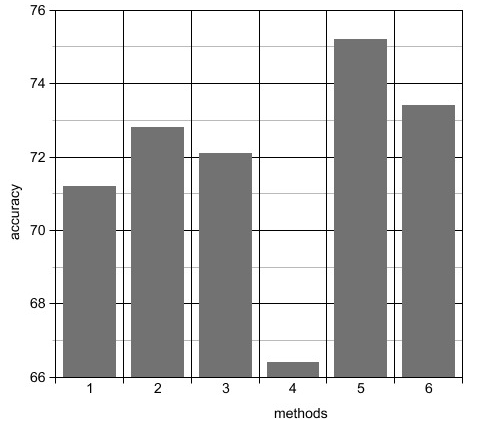
\includegraphics[width=0.5\textwidth]{images/stateoart_acc.png}
	\caption{The Reported Accuracies of models according to state of art}
\end{figure}
\paragraph{}
The biggest bottleneck here according to paper is the dataset as it has an only 35k image with a lot of noise and needs too much preprocessing the quick solution for it is appling data augmentation with different attributes and it not always succeed it may be make things even worse, Read the Paper for more details\cite{state_of_art}.
\paragraph{}
Another model build over state of art try to overcome its discussed problem is applied the model on tensorflow and CNN also work on fer13, it defines a similar method to the final methods with some addition to help improve dataset performance adding Dropout and batch normalization Layers and it uses landmarks and a sliding window Hog as feature extraction(see Figure \ref{amine_arch} to check model architecture). \newline 
\begin{figure}{l}
	\centering
	\includegraphics[width=1.\textwidth]{images/CNN_models_architecture.png}
	\caption{CNN model Architecture}
	\label{amine_arch}
\end{figure}
\subsubsection{SVM}
Also we found an implementation using SVM, it depends actually on extraction features using landmarks and Hog and feeds them to a multi-class SVM classifier, here we can find the different architecture and accuracy of two models based on CNN and SVM model. \ref{amine}

\begin{table}[h!]
	\begin{center}
		\caption{3. Classification Results (training on 5 expressions)\newline}
		\label{amine}
		\begin{tabular}{l|c|l|l}
			\textbf{Experiments} & \textbf{SVM}   & \textbf{Model A}   & \textbf{Model B}  \\
			\hline
			CNN (on raw pixels)	& -----   & 72.4\% & 73.5\% \\ 
			CNN + Face landmarks & 46.9\% &	73.5\% & 74.4\% \\
			CNN + Face landmarks + HOG & 55.0\% & 68.7\% & 73.2\% \\
			CNN + Face landmarks + HOG + sliding window & \textbf{59.4\%} &\textbf{71.4\%}&\textbf{75.1\%}\\
			& & 
		\end{tabular}
		
	\end{center}
\end{table}


\paragraph{} We try this model with this architecture (model B), the same preprocessing and on the same dataset but we get only 50\% testing accuracy.

\subsubsection{Transfer-Learning}
\label{sec:transferlearning}
Transfer learning is a machine learning method where a model developed for a task is reused as the starting point for a model on a second task.
It is a popular approach in deep learning where pre-trained models are used as the starting point on computer vision and natural language processing tasks given the vast compute and time resources required to develop neural network models on these problems and from the huge jumps in skill that they provide on related problems.

In the state of art paper use VGG pretrained model with the architecture CCPCCPCCPCCPFF and get 72.7\% .

